\chapter{La poblaci�n carcelaria en Colombia 1991 - 2017}

\section{An�lisis exploratorio}

El INPEC publica mensualemente la serie poblaci�n carcelaria, desde 1991 hasta el mese anterior a la publicaci�n. Esta serie se encuentra separada por situaci�n jur�dica (condenados, sindicados) y por genero.

La poblaci�n carcelaria total entre 1991 y 2017 se ha cuadruplicado, al pasar de 32.036 a 128.125 internos. Ver figura \ref{fig:genero}.  Aunque la mayor�a de los internos son hombres, la poblaci�n carcelaria femenina ha crecido a un ritmo a�n m�s acelerado, al quintuplicar su poblaci�n entre  1991 y 2017 (pasa de 1633 personas a 7800). 

\begin{figure}[htb]
	\centering
	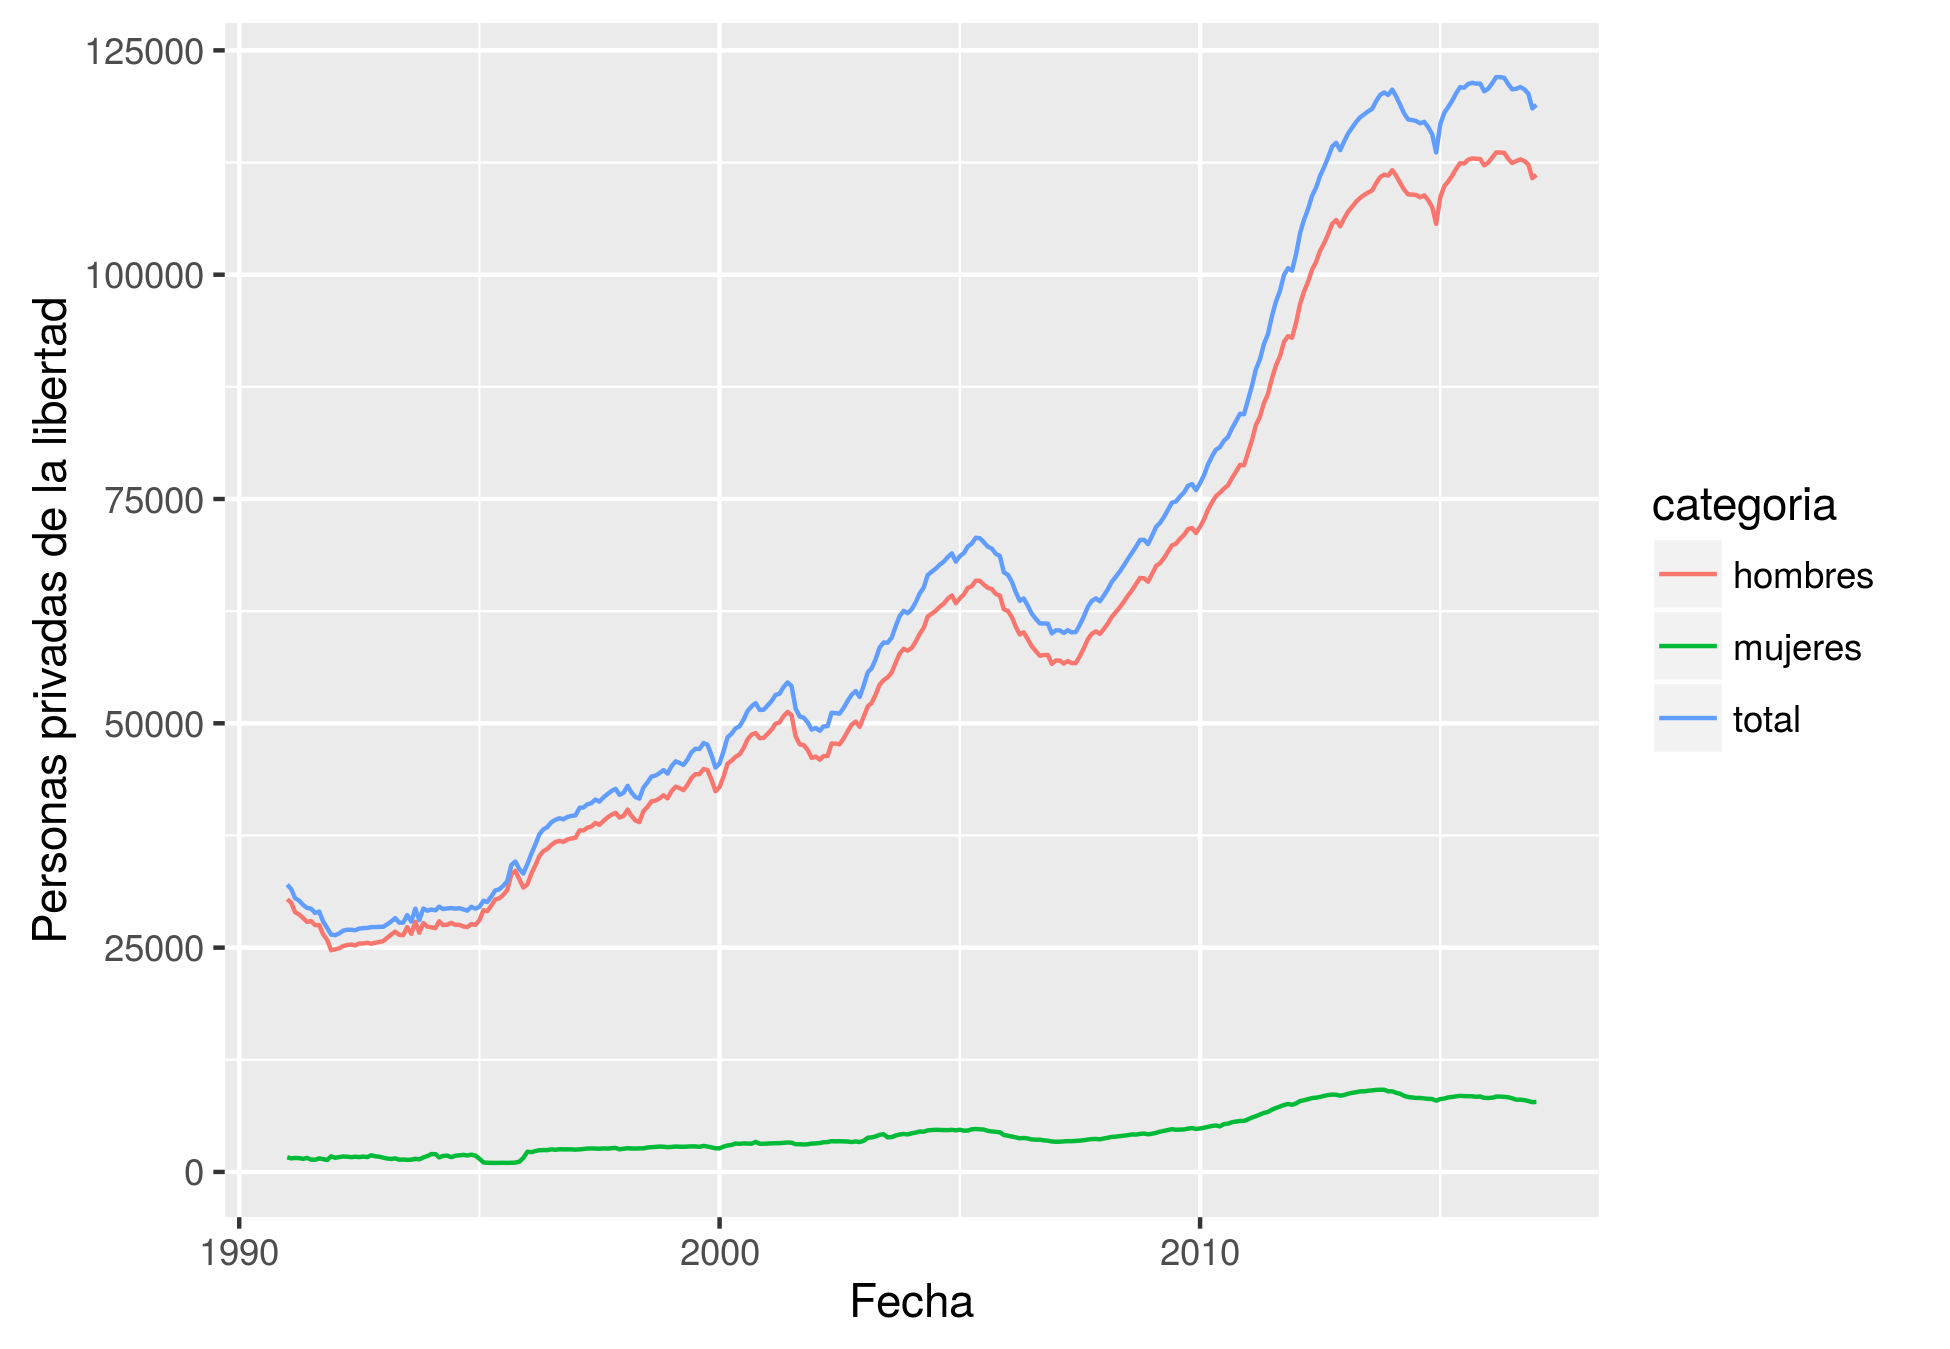
\includegraphics[width=10cm]{genero}
	\caption{Poblaci�n privada de la libertad 1991 - 2017}
	\label{fig:genero}
\end{figure}

El incremento en la poblaci�n carcelaria podr�a tomarse como un efecto del crecimiento de la poblaci�n colombiana. Para validar este supuesto calculamos la tasa de encarcelamiento, que mide la cantidad de personas encarceladas por cada cien mil habitantes. Este indicador pas� de 92 personas por cada cien mil habitantes en enero de 1991 a 242 en enero de 2016. Tal incremento se puede ver tanto en hombres como en mujeres. Ver figura \ref{fig:tasas}. 


\begin{figure}[htb]
	\centering
	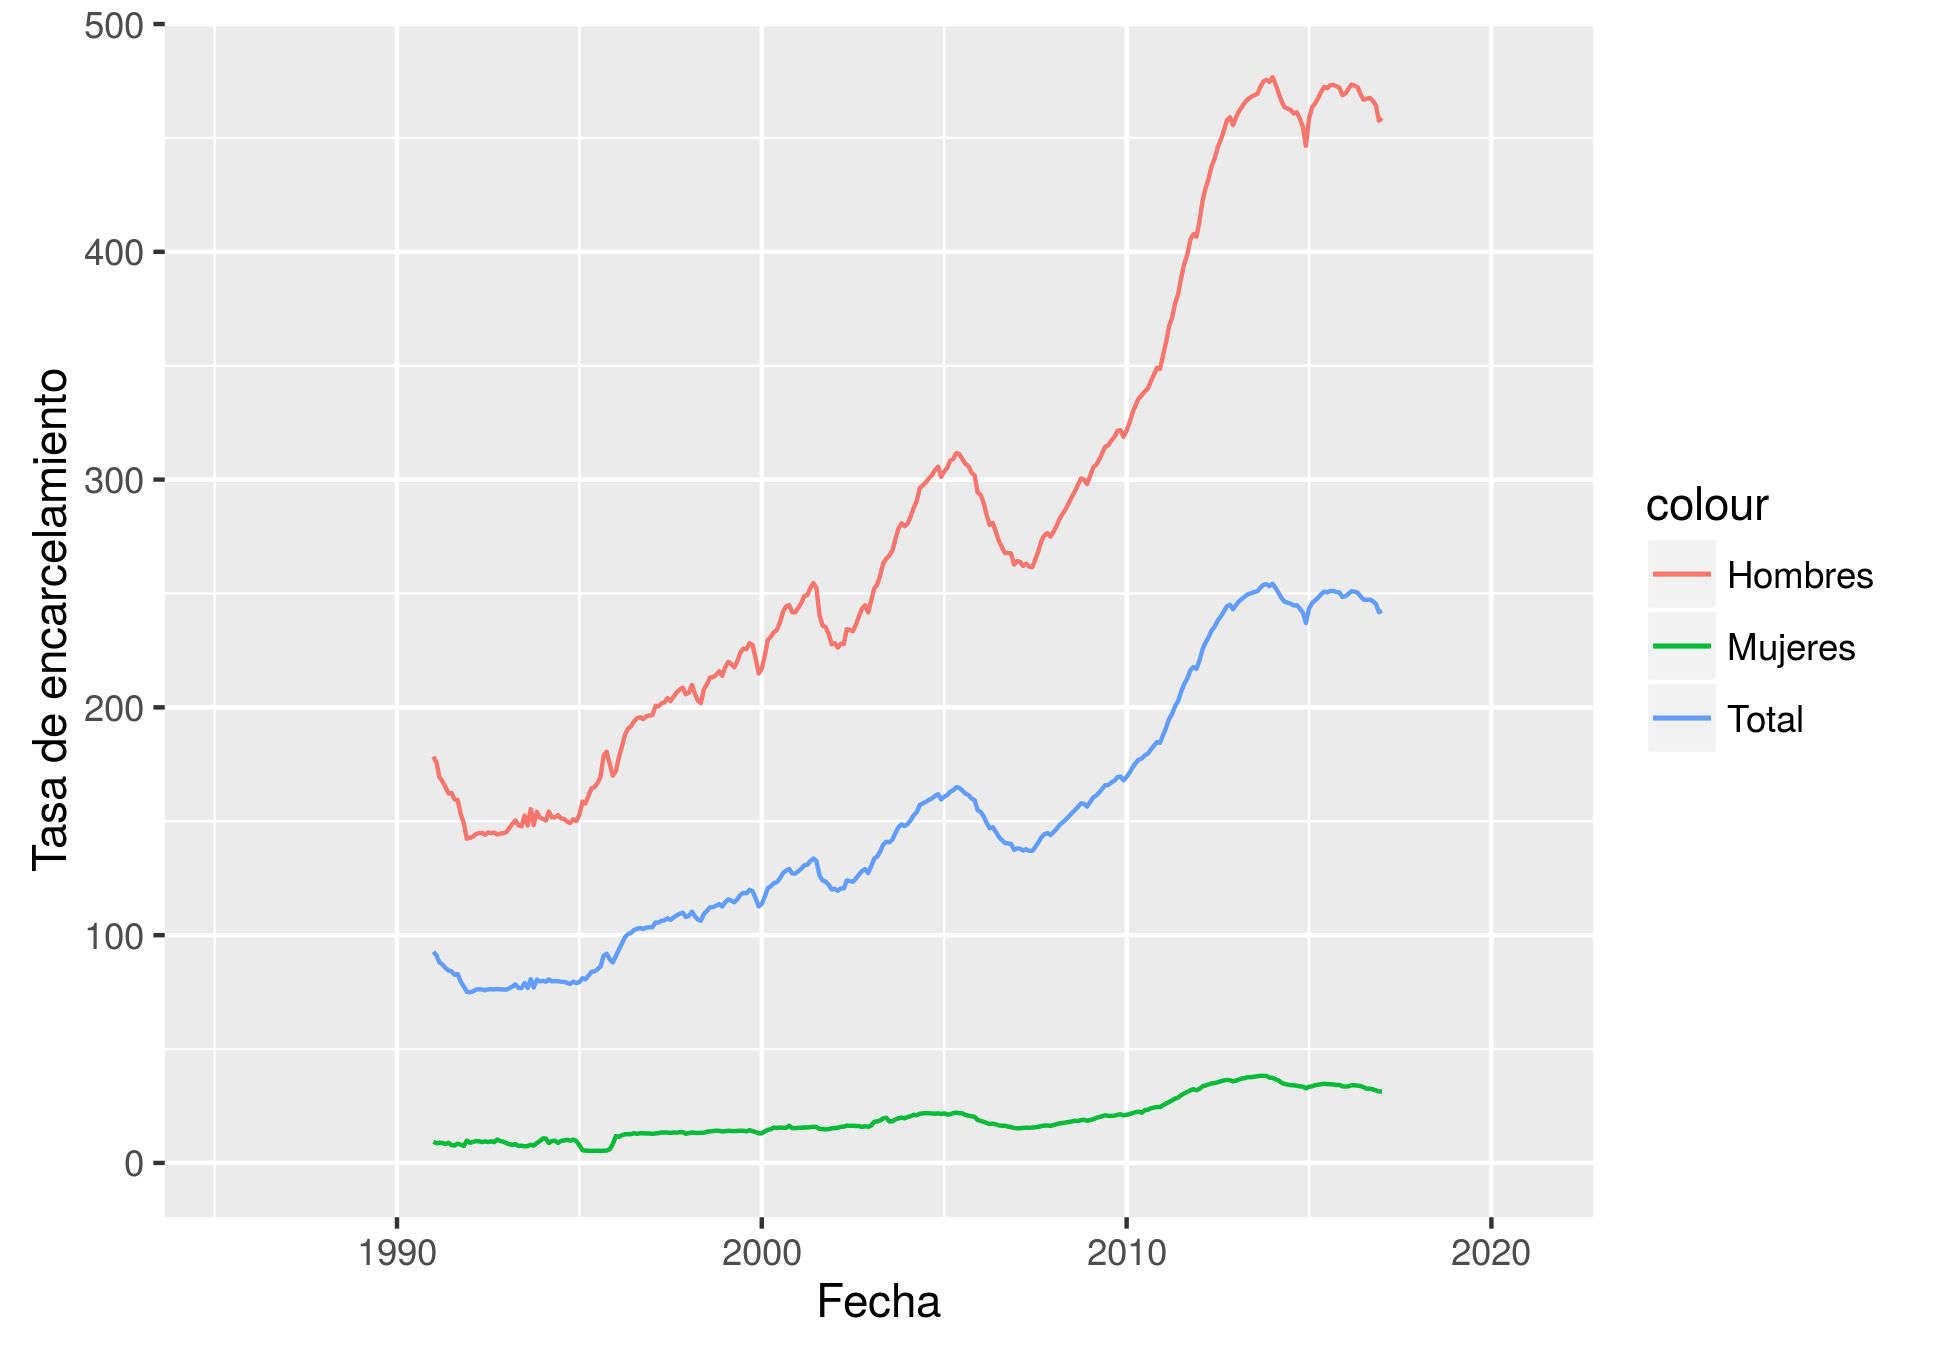
\includegraphics[width=10cm]{tasas}
	\caption{Tasa de encarcelamiento seg�n genero 1991 - 2017 ()}
	\label{fig:tasas}
\end{figure}

\section{El sistema carcelario en Colombia}

\section{Implicaciones en el modelado}